\documentclass[a4paper,12 pt]{article} 
\usepackage[utf8]{inputenc}
\usepackage[T2A]{fontenc}
\usepackage[left=2cm,right=2cm,
top=2cm,bottom=2cm,bindingoffset=0cm]{geometry}
\usepackage{longtable}
\usepackage{lscape}
\usepackage{subcaption}
\usepackage[english,russian]{babel} %локализация
\usepackage{graphicx}%Вставка картинок правильная
\usepackage{float}%"Плавающие" картинки
\usepackage{amsmath, amsfonts, amssymb, amsthm, mathtools} %математика
\begin{document}
 \author{Зажигина Елизавета}
\begin{center}
	Московский физико-технический институт \\*
	\hrulefill
\end{center}

\vspace{8em}

\begin{center}
	\Large Лабораторная работа:
\end{center}

\vspace{2.5em}

\begin{center}
	\textsc{\textbf{Исследование систем массового обслуживания M|M|1|k и M|D|1
			\linebreak}}
\end{center}

\vspace{6em}

\begin{flushleft}
	Студентка \hrulefill Зажигина Е.А \\
	
\end{flushleft}

\vspace{\fill}

\begin{center}
	Март 2021
\end{center}
\newpage
\section*{Постановка задачи:}
В этой лабораторной работе предлагается изучить системы массового обслуживания (далее СМО) $M|M|1|k$ и $M|D|1$, а также сравнить основные характеристики таких систем с теоретическими расчетами: среднее время обслуживания заявки, долю отброшенных пакетов при разных значениях $\lambda, \mu, k$ -- интенсивностях поступления, обработки и длины очереди. 

\section*{Особенности реализации:}
Для исследования этих СМО предполагалось дорабатывать исходный код на языке C++. Для имплементации системы $M|D|1$ подходит дискретное распределение из стандартной библиотеки. Была реализована поддержка конечной и бесконечной очереди для $M|M|1|k$ и $M|D|1$, которая задается при запуске программы: $0$ -- бесконечная очередь, $k > 0$ -- конечная. Также удалось ввести учет отброшенных кадров $PLR$ -- packet loss ratio. Для этой величины также считается доверительный интервал с уровнем доверия 95\%. Сравнение данных происходило в программе на языке Python с помощью графиков. 


\section*{Аналитическая модель:}
Обозначим как $\lambda $ интенсивность поступления заявок в СМО, $\mu$ -- интенсивность их обслуживания, при этом будем полагать, что $\lambda < \mu$. 
СМО $M|M|1$ характеризуется экспоненциальным распределением поступления и обслуживания заявок и одним обслуживающим устройством. В~\cite{kleinrock1975queuing} можно найти выводы этих формул. Для такой системы вероятность находиться в состоянии $k$, где $k$ число заявок в системе определяется:
\begin{equation}
p_k = p_0 (\frac{\lambda}{\mu})^k,
\end{equation}
где $p_0$ -- вероятность того, что в системе нет заявок. С помощью условия нормировки $\sum_i p_i = 1$ можно получить выражение для $p_0$ (при предположении, что $\lambda < \mu$):

\begin{equation}
p_0 = [1 + \sum^{\infty}_{k = 1} (\frac{\lambda}{\mu})^k]^{-1} = 1 - \frac{\lambda}{\mu}.
\end{equation}
Среднее число заявок с системе $\bar{N}$, обозначив $\frac{\lambda}{\mu} = \rho$, находится как:
\begin{equation}
	\bar{N} = \sum^{\infty}_{k = 0}p_k \cdot k = (1-\rho) \sum^{\infty}_{k = 0} k\rho^k = (1-\rho)\rho\frac{\partial}{\partial\rho}(1/(1-\rho)) =  \frac{\frac{\lambda}{\mu}}{1-\frac{\lambda}{\mu}}.
\end{equation}
По формуле Литтла можно найти и среднее время $T$, когда заявка находится в системе:
\begin{equation}
T_s = \frac{\bar{N}}{\lambda}.
\end{equation}
В системе $M|M|1|K$ присутствует конечный накопитель размера $K$. Модифицируем формулы выше. В систему допускаются только те требования, который застают в ней строго меньше, чем $K$ требований. Поэтому вероятность состояний $p_k$ и $p_0$ (определяется из условия нормировки), $\rho = \frac{\lambda}{\mu}$:
\begin{equation}
p_k =  p_0 \Pi^{k - 1}_{i = 0}\frac{\lambda_i}{\mu_{i+1}} = 	\begin{cases} p_0(\frac{\lambda}{\mu})^{k} = \frac{1 - \frac{\lambda}{\mu}}{1-(\frac{\lambda}{\mu})^{k + 1}}(\frac{\lambda}{\mu})^k,  & \text{если } 0 \le k \le K; \\
0, & \text{в остальных случаях. } \\
	\end{cases}
\end{equation}
\begin{equation}
	p_0 = [1 + \frac{\rho(1-\rho^K)}{1-\rho}]^{-1}.
\end{equation}
Вероятность  отказа в обслуживании определяется в том случае, когда в системе одно требование находится в обслуживающем приборе и $K-1$ требований в накопителе (в очереди):
\begin{equation}
	P_{\text{отк}} = p_k.
\end{equation}
Средний размер очереди $\bar{N}$ считаем как матожидание длины очереди:
\begin{equation}
	\bar{N} = \sum^{K}_{k = 1}p_k \cdot k,
\end{equation} 
а среднее время пребывания в системе как:
\begin{equation}
	T_s = \frac{\bar{N}}{\lambda \cdot (1 - P_{\text{отк}})}.
\end{equation}
СМО $M|D|1$ характеризуется экспоненциальным поступлением заявок, детерминированным временем обслуживания одной заявки и одним обслуживающим устройством. Воспользуемся формулой Полячека-Хинчина для системы $M|G|1$, где $G$ -- произвольное распределение обслуживания заявок. Считаем известным, что среднее число заявок $\bar{q}$ в такой системе определяется: 
\begin{equation}
	\bar{q} = \rho + \frac{\lambda^2 \bar{x^2}}{2 (1-\rho)} = \rho + \rho^2\frac{1 + C^2_b}{2 (1-\rho)},
\end{equation}
где $\bar{x^2}$ -- второй момент распределения времени обслуживания, $\rho = \lambda \bar{x}$, $C^2_b = \frac{\varsigma^2_b}{\bar{x^2}}$ -- нормированная дисперсия времени обслуживания. Так как в $M|D|1$ время обслуживания детерминировано, то $C^2_b = 0$.
Для такой системы среднее время нахождения в системе $T_s$ (пользуясь законом Литтла):
\begin{equation}
	T_s = \dfrac{\rho}{2\mu(1-\rho)} + \frac{1}{\mu},
\end{equation}
где $\rho = \frac{\lambda}{\mu}$. 

\section*{Результаты:}
В результате моделирования системы $M|M|1|k$ были получены семейства кривых, представленные на рис.~\ref{fig:mm1k}. С ростом $\frac{\lambda}{\mu}$ очередь заполняется быстрее, поэтому растет и вероятность отказа в обслуживании. Очевидно, что увеличение размера очереди снижает вероятность отказа, но в то же время при большом $\frac{\lambda}{\mu}$ среднее время обслуживания растет из-за того, что обслуживать может только одно устройство и оно не успевает справляться со всеми заявками быстро, но этого хватает, чтобы доля отказанных была небольшой.

Для $M|D|1$ исследовалась система с бесконечной очередью. На рис.~\ref{fig:md1} представлено сравнение двух обслуживающих систем: $M|D|1$ и $M|M|1$. Видно, что быстрее обслуживает система с детерминированным временем обработки заявки. 

На обоих графиках~\ref{fig:mm1k} и~\ref{fig:md1} видно хорошее согласование теоретических расчетов и имитационного моделирования систем.
\begin{figure}[H]%[tb]
	\begin{subfigure}{\textwidth}
		\center{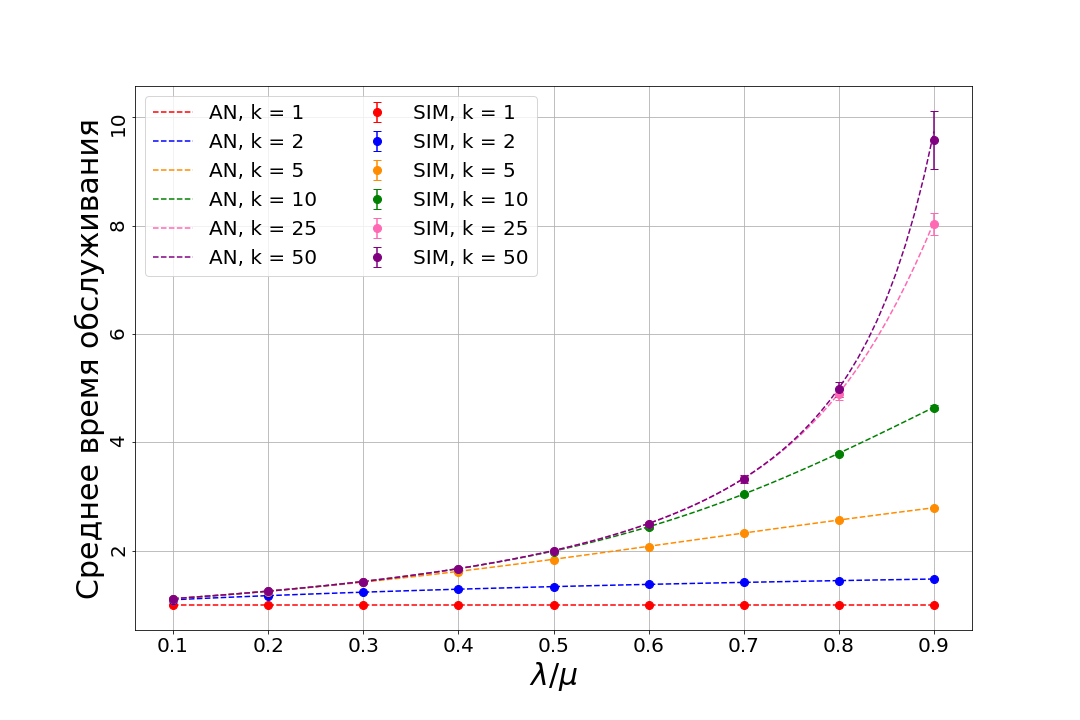
\includegraphics[width=\linewidth]{pics/service_time_MM1.png}}
		\caption{}
	\end{subfigure}
	\hspace{\fill}%
	\begin{subfigure}{\textwidth}
		\center{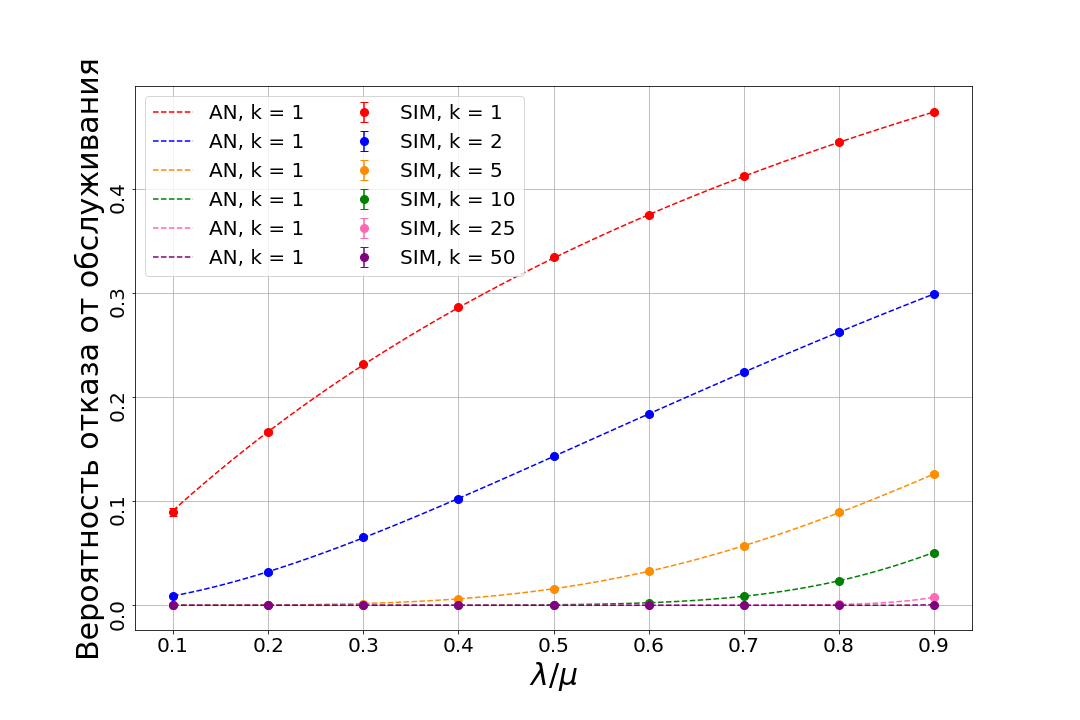
\includegraphics[width=\linewidth]{pics/plr_MM1.png}}
		\caption{}
	\end{subfigure}
	\caption{Семейство зависимостей характеристик системы $M|M|1|k $ от параметров входного потока при разных значениях длины очереди $k$. Зависимость \textbf{(a)} среднего времени обслуживания и \textbf{(b)} и доли отброшенных заявок от $\frac{\lambda}{\mu}$. $AN$ и $SIM$ соответствуют аналитическому расчету и имитационному моделированию.}
	\label{fig:mm1k}
\end{figure}

\begin{figure}[H]%[tb]
	\center{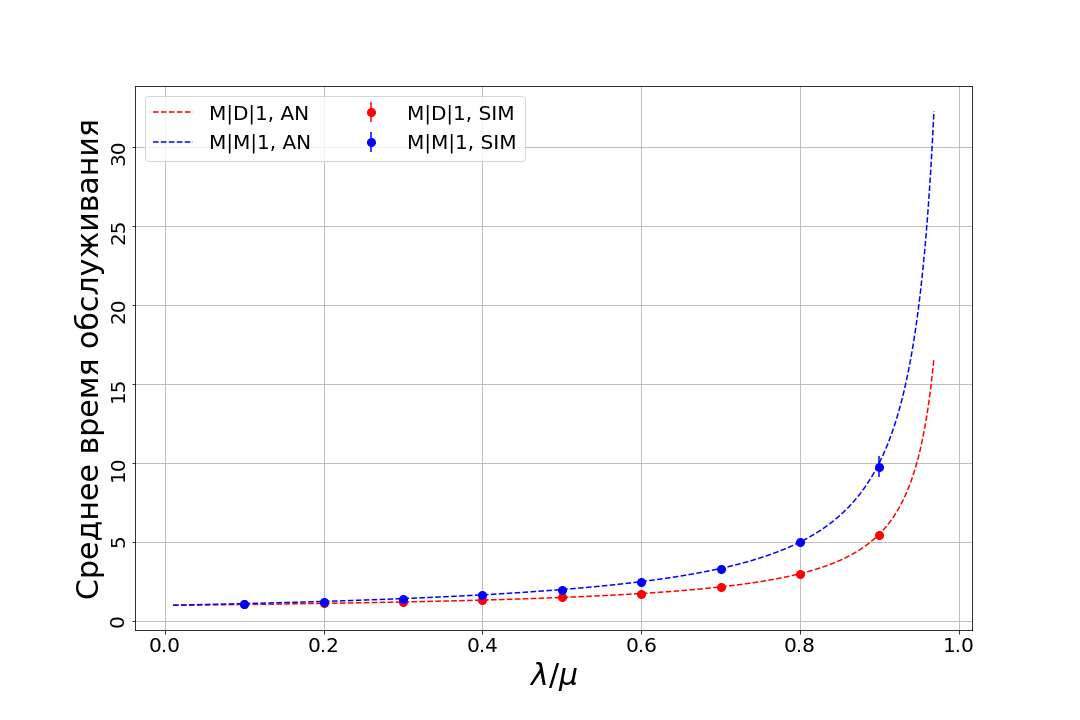
\includegraphics[width=\linewidth]{pics/service_time_MD1.png}}
	\caption{Зависимость среднего времени обслуживания от $\frac{\lambda}{\mu}$ для СМО $M|D|1$ и $M|M|1$. $AN$ и $SIM$ соответствуют аналитическому расчету и имитационному моделированию.}
	\label{fig:md1}
\end{figure}
\section*{Выводы:}
В данной работе предлагалось изучить СМО $M|D|1|$ и $M|M|1$. На основании теоретический расчетов и имитационного моделирования нам удалось сравнить характеристики этих двух систем.
\addcontentsline{toc}{section}{Bibliography}
\bibliographystyle{ugost2008}
\bibliography{biblio}
\end{document}